\documentclass{deltares_manual}

\usepackage{tikz}
\usepackage[pipeTables=true]{markdown}

%------------------------------------------------------------------------------
\newcommand{\dfastbe}{\textrm{D-FAST~Bank~Erosion}\xspace}

\hypersetup
{
    pdfauthor   = {Deltares},
    pdftitle    = {\dfastbe},
    pdfkeywords = {Deltares User Manual \dfastbe}
}

%------------------------------------------------------------------------------
%

%\makeindex

%------------------------------------------------------------------------------
%
\begin{document}
\pagestyle{empty}
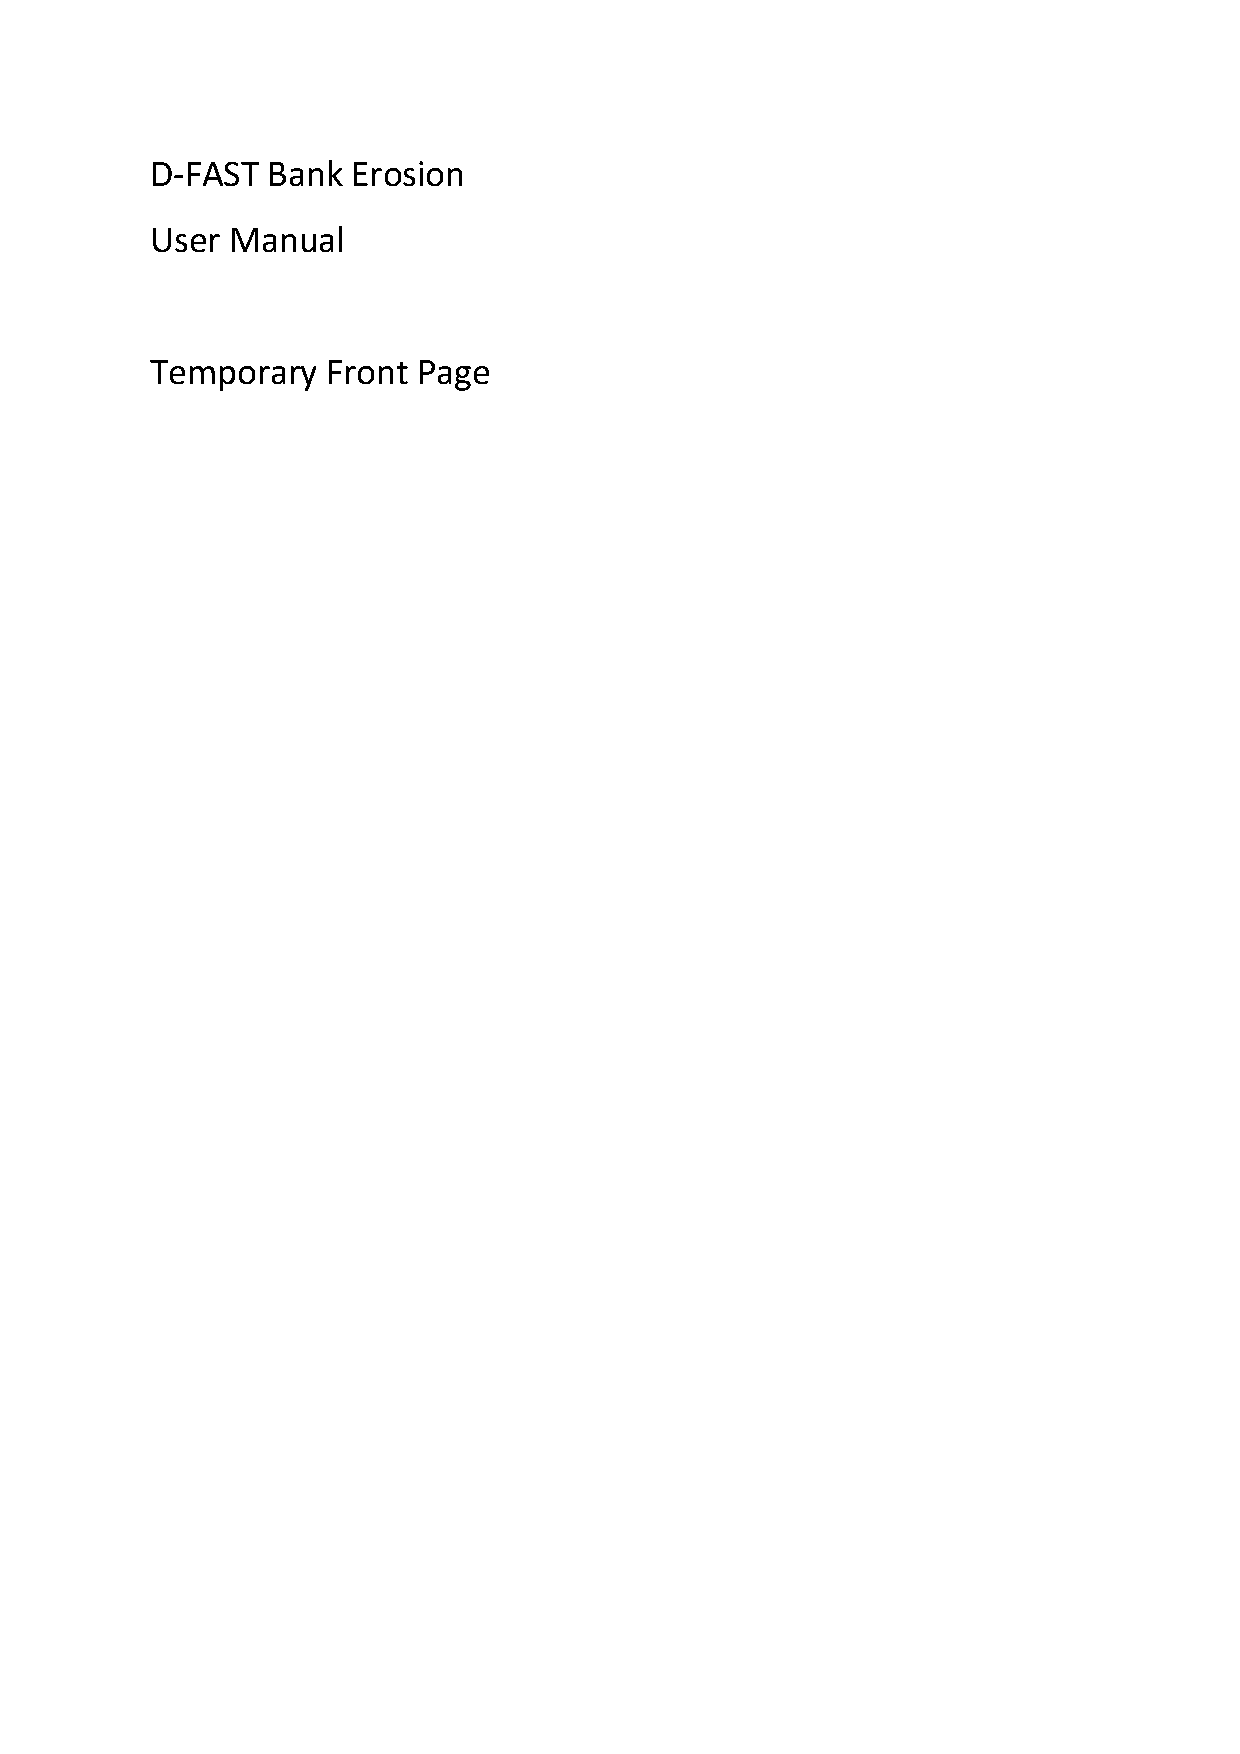
\includepdf[pages=1, offset=72 -70]{cover/d-fast-bank-erosion.pdf} % links-rechts past precies
\cleardoublepage
\title{\dfastbe}
\subtitle{}
\manualtype{User Manual}
\version{0.1}

\author{ }

\deltarestitle
%
\markdownInput{../userman.md}
\chapter{Conceptual description}
\markdownInput{../techref/techref.md}
%\textit{}\chapter{A guide to this manual} \label{Chp:Guide}

\section{Introduction}
This User Manual describes the theory and usage of \dfastbe.
This rapid assessment tool for bank erosion along rivers has been designed to work with simulation results obtained from \dflowfm, but can also applied using results from \dflow or WAQUA.

\section{Overview}
This manual is split in the following sections

\begin{itemize}
\item \Autoref{Chp:Guide}, i.e.~this chapter, gives a general overview of the manual,
\item \Autoref{Chp:Introduction} introduces the general concepts of \dfastbe and describes its application domain,
\item \Autoref{Chp:GetStarted} describes briefly how to install and use \dfastbe,
%\item \Autoref{Chp:Tutorial} ...
\item \Autoref{Chp:BankDetect} describes the bank line detection algorithm,
\item \Autoref{Chp:BankErosion} describes the bank erosion concepts implemented,
\item \Autoref{bankcomp} gives an overview of characteristic bank strength values,
\item \Autoref{Chp:FileFormats} describes the file formats used by the software.
\end{itemize}

\section{Typographical conventions}
Throughout this manual, the following conventions help you to distinguish between different elements of text.

\begin{longtable*}{p{2.0in}|p{\textwidth-2.0in-12pt}}
Example \STRUT & Description \\ \hline \endhead
<mydir \textbackslash usecase.cfg> \STRUT &
Directory names, filenames, and path names are expressed between angle brackets, <>. \\
“27 08 1999” \STRUT &
Data to be typed by you into the input fields are displayed between double quotes.
Selections of menu items, option boxes etc. are described as such: for instance 'select Save and go to the next window'. \\
\command{dfastbe} \STRUT &
Commands to be typed by you are given in the font Courier New, 10 points. \\
%\includegraphics[height=4mm]{pictures/action_arrow.pdf} \STRUT &
% In the Tutorial, user actions are indicated with this arrow. \\
\unitbrackets{\si{\meter\per\second}} \unitbrackets{\si{-}} \STRUT &
Units are given between square brackets when used next to the formulae. Leaving them out might result in misinterpretation.
Most units will be in SI notation.
\unitbrackets{m AD} stands for 'meter Above Datum', which denotes a level relative to the vertical reference system.
\end{longtable*}

Command prompts, file listings and terminal output are shown in typewriter font:

\begin{Verbatim}
> dfastbe --mode banklines
=====================================================
Determine bank lines
=====================================================
version: D-FAST Bank Erosion 2.1.0
source: https://github.com/Deltares/D-FAST_Bank_Erosion
-----------------------------------------------------
saving output in directory: output\banklines
reading chainage information from file : inputfiles\rivkm_20m.xyc
clipping chainage to the range 123.0 to 128.0 km
reading search line 1 from file : inputfiles\oeverlijn_links_mod.xyc
reading search line 2 from file : inputfiles\oeverlijn_rechts_mod.xyc
-----------------------------------------------------
reading simulation data from : sim270\SDS-j19_map.nc
-----------------------------------------------------
importing grid...
importing bathymetry ...
importing water level ...

... continued ...
\end{Verbatim}


%\nonumchapter{References}
%\bibliography{../common/deltares_manual}

%\appendix

%\include{chapters_usermanual/appmdufile}

\pagestyle{empty}
\cleardoublepage
\mbox{}
\includepdf[pages=2, offset=-72 -70]{cover/d-fast-bank-erosion.pdf} % links-rechts past precies
\end{document}
